\documentclass[border=8pt, multi, tikz]{standalone}
%\usepackage{blocks}
\usepackage{import}
\subimport{}{init}
\usetikzlibrary{positioning}
\usetikzlibrary{3d}

\def\ConvColor{rgb:yellow,5;red,2.5;white,5}
\def\ConvReluColor{rgb:yellow,5;red,5;white,5}
\def\PoolColor{rgb:red,1;black,0.3}
\def\UnpoolColor{rgb:blue,2;green,1;black,0.3}
\def\FcColor{rgb:blue,5;red,2.5;white,5}
\def\FcReluColor{rgb:blue,5;red,5;white,4}
\def\SoftmaxColor{rgb:magenta,5;black,7}


\newcommand{\copymidarrow}{\tikz \draw[-Stealth,line width =0.8mm,draw={rgb:blue,4;red,1;green,1;black,3}] (-0.3,0) -- ++(0.3,0);}

\begin{document}
\begin{tikzpicture}
\tikzstyle{connection}=[ultra thick,every node/.style={sloped,allow upside down},draw=\edgecolor,opacity=0.7]
\tikzstyle{copyconnection}=[ultra thick,every node/.style={sloped,allow upside down},draw={rgb:blue,4;red,1;green,1;black,3},opacity=0.7]

%%%%%%%%%%%%%%%%%%%%%%%%%%%%%%%%%%%%%%%%%%%%%%%%%%%%%%%%%%%%%%%%%%%%%%%%%%%%%%%%%%%%%%%%
%% Draw Encoder
%%%%%%%%%%%%%%%%%%%%%%%%%%%%%%%%%%%%%%%%%%%%%%%%%%%%%%%%%%%%%%%%%%%%%%%%%%%%%%%%%%%%%%%%
% Pre disaster
\node[canvas is zy plane at x=0] (temp) at (-3,0,0) {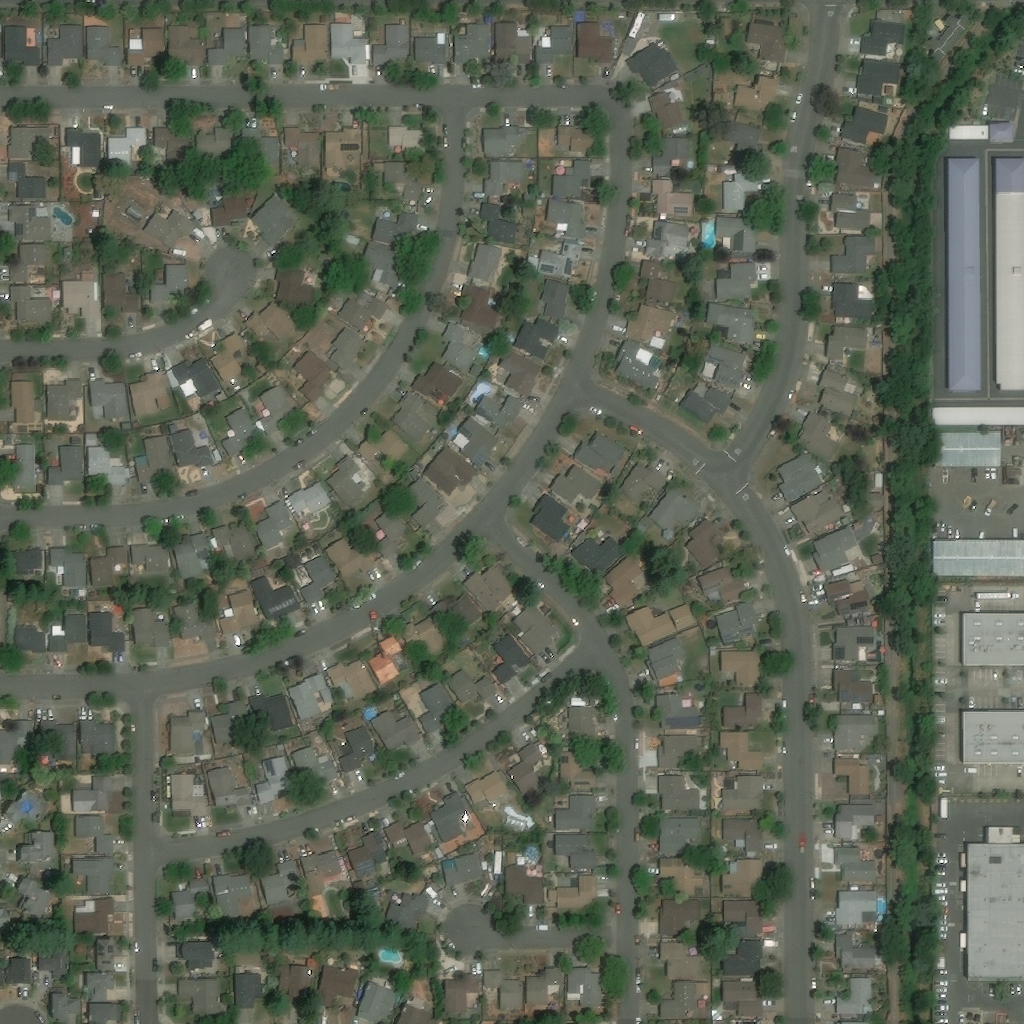
\includegraphics[width=8cm,height=8cm]{santa-rosa-wildfire_00000161_pre_disaster.png}};

% Post disaster
\node[canvas is zy plane at x=0] (temp) at (-3,12,0) {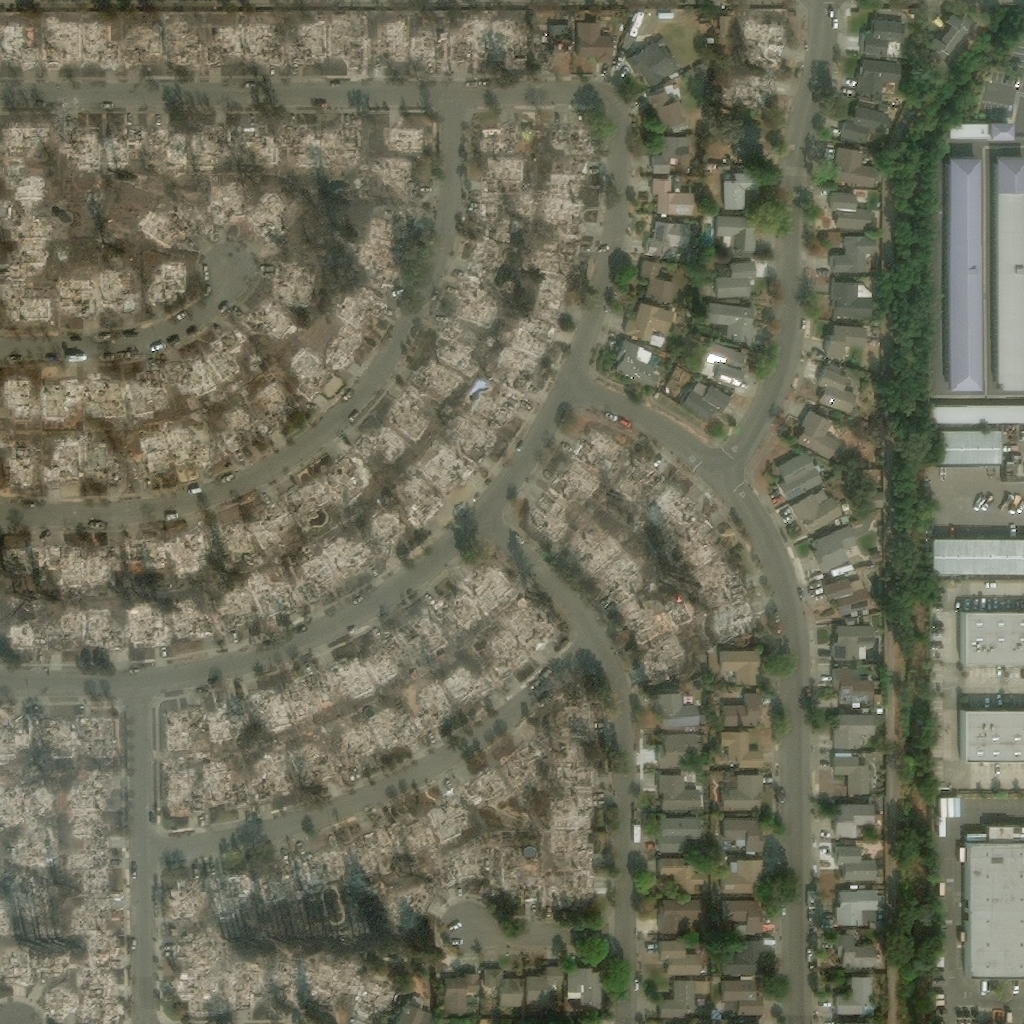
\includegraphics[width=8cm,height=8cm]{santa-rosa-wildfire_00000161_post_disaster.png}};

% Input A Encoder
            
% a_conv1_1, a_conv1_2
\pic[shift={(0,0,0)}] at (0,0,0) {RightBandedBox={name=a_cr1,%
        xlabel={{"16","32"}},zlabel=I,fill=\ConvColor,bandfill=\ConvReluColor,%
        height=40,width={2,2},depth=40}};
%pool1
\pic[shift={(0,0,0)}] at (a_cr1-east) {Box={name=a_p1,%
        fill=\PoolColor,opacity=0.5,height=32,width=1,depth=32}};
%%%%%%%%%%
% conv2_1,conv2_2
\pic[shift={(1,0,0)}] at (a_p1-east) {RightBandedBox={name=a_cr2,%
        xlabel={{"64","64"}},zlabel=I/2,fill=\ConvColor,bandfill=\ConvReluColor,%
        height=32,width={3.5,3.5},depth=32}};
%pool2
\pic[shift={(0,0,0)}] at (a_cr2-east) {Box={name=a_p2,%
        fill=\PoolColor,opacity=0.5,height=25,width=1,depth=25}};
%%%%%%%%%%
% conv3_1,conv3_2
\pic[shift={(0.75,0,0)}] at (a_p2-east) {RightBandedBox={name=a_cr3,%
        xlabel={{"128","128"}},zlabel=I/4,fill=\ConvColor,bandfill=\ConvReluColor,%
        height=25,width={4.5,4.5},depth=25}};
%pool3
\pic[shift={(0,0,0)}] at (a_cr3-east) {Box={name=a_p3,%
        fill=\PoolColor,opacity=0.5,height=16,width=1,depth=16}};
%%%%%%%%%%
% conv4_1,conv4_2,conv4_3
\pic[shift={(0.5,0,0)}] at (a_p3-east) {RightBandedBox={name=a_cr4,%
        xlabel={{"256","256"}},zlabel=I/8,fill=\ConvColor,bandfill=\ConvReluColor,%
        height=16,width={6,6},depth=16}};
%pool4
\pic[shift={(0,0,0)}] at (a_cr4-east) {Box={name=a_p4,%
        fill=\PoolColor,opacity=0.5,height=8,width=1,depth=8}};
        
%%%%%%%%%%%%%%%%%%%%%%%%%%%%%%%%%%%%%%%%%%%%%%%%%%%%%%%%%%%%%%%%%%%%%%%%%%%%%%%%%%%%%%%%
      
% Input B Encoder

% a_conv1_1,a_conv1_2
\pic[shift={(0,12,0)}] at (0,0,0) {RightBandedBox={name=b_cr1,%
        xlabel={{"16","32"}},zlabel=I,fill=\ConvColor,bandfill=\ConvReluColor,%
        height=40,width={2,2},depth=40}};
%a_pool1
\pic[shift={(0,0,0)}] at (b_cr1-east) {Box={name=b_p1,%
        fill=\PoolColor,opacity=0.5,height=32,width=1,depth=32}};
   
%%%%%%%%%%
% a_conv2_1, a_conv2_2
\pic[shift={(1,0,0)}] at (b_p1-east) {RightBandedBox={name=b_cr2,%
        xlabel={{"64","64"}},zlabel=I/2,fill=\ConvColor,bandfill=\ConvReluColor,%
        height=32,width={3.5,3.5},depth=32}};
% a_pool2
\pic[shift={(0,0,0)}] at (b_cr2-east) {Box={name=b_p2,%
        fill=\PoolColor,opacity=0.5,height=25,width=1,depth=25}};
        
%%%%%%%%%%
% a_conv3_1, a_conv3_2
\pic[shift={(0.75,0,0)}] at (b_p2-east) {RightBandedBox={name=b_cr3,%
        xlabel={{"128","128"}},zlabel=I/4,fill=\ConvColor,bandfill=\ConvReluColor,%
        height=25,width={4.5,4.5},depth=25}};
% a_pool3
\pic[shift={(0,0,0)}] at (b_cr3-east) {Box={name=b_p3,%
        fill=\PoolColor,opacity=0.5,height=16,width=1,depth=16}};

%%%%%%%%%%
% a_conv4_1, a_conv4_2, conv4_3
\pic[shift={(0.5,0,0)}] at (b_p3-east) {RightBandedBox={name=b_cr4,%
        xlabel={{"256","256"}},zlabel=I/8,fill=\ConvColor,bandfill=\ConvReluColor,%
        height=16,width={6,6},depth=16}};
%pool4
\pic[shift={(0,0,0)}] at (b_cr4-east) {Box={name=b_p4,%
        fill=\PoolColor,opacity=0.5,height=8,width=1,depth=8}};
%%%%%%%%%%%%%%%%%%%%%%%%%%%%%%%%%%%%%%%%%%%%%%%%%%%%%%%%%%%%%%%%%%%%%%%%%%%%%%%%%%%%%%%%
%% Bottleneck
%%%%%%%%%%%%%%%%%%%%%%%%%%%%%%%%%%%%%%%%%%%%%%%%%%%%%%%%%%%%%%%%%%%%%%%%%%%%%%%%%%%%%%%%% conv5_1,conv5_2,conv5_3
\pic[shift={(0.75,0,0)}] at (a_p4-east) {RightBandedBox={name=cr5,caption=Bottleneck Conv,%
        xlabel={{"512","512"}},zlabel=I/16,fill=\ConvColor,bandfill=\ConvReluColor,%
        height=8,width={8,8},depth=8}};
%%%%%%%%%%%%%%%%%%%%%%%%%%%%%%%%%%%%%%%%%%%%%%%%%%%%%%%%%%%%%%%%%%%%%%%%%%%%%%%%%%%%%%%%
%% Draw Decoder 
%%%%%%%%%%%%%%%%%%%%%%%%%%%%%%%%%%%%%%%%%%%%%%%%%%%%%%%%%%%%%%%%%%%%%%%%%%%%%%%%%%%%%%%%
%% unpool4, 
\pic[shift={(1.2,0,0)}] at (cr5-east) {Box={name=up4,%
        fill=\UnpoolColor,opacity=0.6,height=16,width=1,depth=16}};
\pic[shift={(0,0,0)}] at (up4-east) {RightBandedBox={name=ucr4,%
        xlabel={{"256","dummy"}},fill=\ConvColor,bandfill=\ConvReluColor,%
        height=16,width=6,depth=16}};
\pic[shift={(0,0,0)}] at (ucr4-east) {RightBandedBox={name=cat4,%
        xlabel={{"256",""}},fill={rgb:white,1;black,3},bandfill={rgb:white,1;black,2},opacity=0.2,height=16,width=6,depth=16}};    
\pic[shift={(0,0,0)}] at (cat4-east) {RightBandedBox={name=ucr4a,%
        xlabel={{"256","256"}},zlabel=I/8,fill=\ConvColor,bandfill=\ConvReluColor,%
        height=16,width={6,6},depth=16}};
%%%%%%%%%%
%% unpool3, 
\pic[shift={(1.5,0,0)}] at (ucr4a-east) {Box={name=up3,%
        fill=\UnpoolColor,opacity=0.6,height=25,width=1,depth=25}};
\pic[shift={(0,0,0)}] at (up3-east) {RightBandedBox={name=ucr3,%
        xlabel={{"128","dummy"}},fill=\ConvColor,bandfill=\ConvReluColor,%
        height=25,width=4.5,depth=25}};
\pic[shift={(0,0,0)}] at (ucr3-east) {RightBandedBox={name=cat3,%
        xlabel={{"128",""}},fill={rgb:white,1;black,3},bandfill={rgb:white,1;black,2},opacity=0.2,height=25,width=4.5,depth=25}};
\pic[shift={(0,0,0)}] at (cat3-east) {RightBandedBox={name=ucr3a,%
        xlabel={{"128","128"}},zlabel=I/4,fill=\ConvColor,bandfill=\ConvReluColor,%
        height=25,width={4.5,4.5},depth=25}};
%%%%%%%%%%
%% unpool2, 
\pic[shift={(1,0,0)}] at (ucr3a-east) {Box={name=up2,%
        fill=\UnpoolColor,opacity=0.6,height=32,width=1,depth=32}};
\pic[shift={(0,0,0)}] at (up2-east) {RightBandedBox={name=ucr2,%
        xlabel={{"64","dummy"}},fill=\ConvColor,bandfill=\ConvReluColor,%
        height=32,width=3.5,depth=32}};
\pic[shift={(0,0,0)}] at (ucr2-east) {RightBandedBox={name=cat2,%
        xlabel={{"64",""}},fill={rgb:white,1;black,3},bandfill={rgb:white,1;black,2},opacity=0.2,height=32,width=3.5,depth=32}};    
\pic[shift={(0,0,0)}] at (cat2-east) {RightBandedBox={name=ucr2a,%
        xlabel={{"64","64"}},zlabel=I/2,fill=\ConvColor,bandfill=\ConvReluColor,%
        height=32,width={3.5,3.5},depth=32}};
%%%%%%%%%%
%% unpool1, 
\pic[shift={(1.5,0,0)}] at (ucr2a-east) {Box={name=up1,%
        fill=\UnpoolColor,opacity=0.6,height=40,width=1,depth=40}};
\pic[shift={(0,0,0)}] at (up1-east) {RightBandedBox={name=ucr1,%
        xlabel={{"32","dummy"}},fill=\ConvColor,bandfill=\ConvReluColor,%
        height=40,width=2.5,depth=40}};
\pic[shift={(0,0,0)}] at (ucr1-east) {RightBandedBox={name=cat1,%
        xlabel={{"32",""}},fill={rgb:white,1;black,3},bandfill={rgb:white,1;black,2},opacity=0.2,height=40,width=2.5,depth=40}};  
\pic[shift={(0,0,0)}] at (cat1-east) {RightBandedBox={name=ucr1a,%
        xlabel={{"32","32"}},fill=\ConvColor,bandfill=\ConvReluColor,%
        height=40,width={2.5,2.5},depth=40}};
%%%%%%%%%%%%%%%%%%%%%%%%%%%%%%%%%%%%%%%%%%%%%%%%%%%%%%%%%%%%%%%%%%%%%%%%%%%%%%%%%%%%%%%%
%% Classifier 
%%%%%%%%%%%%%%%%%%%%%%%%%%%%%%%%%%%%%%%%%%%%%%%%%%%%%%%%%%%%%%%%%%%%%%%%%%%%%%%%%%%%%%%%%
\pic[shift={(0.75,0,0)}] at (ucr1a-east) {Box={name=out,caption=Softmax,%
        zlabel=I,fill=\SoftmaxColor,height=40,width=1,depth=40}};
%%%%%%%%%%%%%%%%%%%%%%%%%%%%%%%%%%%%%%%%%%%%%%%%%%%%%%%%%%%%%%%%%%%%%%%%%%%%%%%%%%%%%%%
% Draw connections
%%%%%%%%%%%%%%%%%%%%%%%%%%%%%%%%%%%%%%%%%%%%%%%%%%%%%%%%%%%%%%%%%%%%%%%%%%%%%%%%%%%%%%%
\draw [connection]  (a_p1-east)    -- node {\midarrow} (a_cr2-west);
\draw [connection]  (a_p2-east)    -- node {\midarrow} (a_cr3-west);
\draw [connection]  (a_p3-east)    -- node {\midarrow} (a_cr4-west);
\draw [connection]  (a_p4-east)    -- node {\midarrow} (cr5-west);
\draw [connection]  (cr5-east)   -- node {\midarrow} (up4-west);
\draw [connection]  (ucr4a-east) -- node {\midarrow} (up3-west);
\draw [connection]  (ucr3a-east) -- node {\midarrow} (up2-west);
\draw [connection]  (ucr2a-east) -- node {\midarrow} (up1-west);
\draw [connection]  (ucr1a-east) -- node {\midarrow} (out-west);
%\draw [connection]  (out-east)   -- node {\midarrow} ++(2,0,0);

\draw [connection]  (b_p1-east)    -- node {\midarrow} (b_cr2-west);
\draw [connection]  (b_p2-east)    -- node {\midarrow} (b_cr3-west);
\draw [connection]  (b_p3-east)    -- node {\midarrow} (b_cr4-west);


\path (a_cr4-southeast) -- (a_cr4-northeast) coordinate[pos=1.25] (a_cr4-top) ;
\path (a_cr3-southeast) -- (a_cr3-northeast) coordinate[pos=1.25] (a_cr3-top) ;
\path (a_cr2-southeast) -- (a_cr2-northeast) coordinate[pos=1.25] (a_cr2-top) ;
\path (a_cr1-southeast) -- (a_cr1-northeast) coordinate[pos=1.25] (a_cr1-top) ;

\path (cat4-south)  -- (cat4-north)  coordinate[pos=1.25] (cat4-top) ;
\path (cat3-south)  -- (cat3-north)  coordinate[pos=1.25] (cat3-top) ;
\path (cat2-south)  -- (cat2-north)  coordinate[pos=1.25] (cat2-top)  ;
\path (cat1-south)  -- (cat1-north)  coordinate[pos=1.25] (cat1-top)  ;


%
\draw [copyconnection]  (a_cr4-northeast)  
-- node {\copymidarrow}(a_cr4-top)
-- node {\copymidarrow}(cat4-top)
-- node {\copymidarrow} (cat4-north);
%
\draw [copyconnection]  (a_cr3-northeast)  
-- node {\copymidarrow}(a_cr3-top)
-- node {\copymidarrow}(cat3-top)
-- node {\copymidarrow} (cat3-north);
%
\draw [copyconnection]  (a_cr2-northeast)  
-- node {\copymidarrow}(a_cr2-top)
-- node {\copymidarrow}(cat2-top)
-- node {\copymidarrow} (cat2-north);
%
\draw [copyconnection]  (a_cr1-northeast)  
-- node {\copymidarrow}(a_cr1-top)
-- node {\copymidarrow}(cat1-top)
-- node {\copymidarrow} (cat1-north);

\path (b_cr4-southeast) -- (b_cr4-northeast) coordinate[pos=1.25] (b_cr4-top) ;
\path (b_cr3-southeast) -- (b_cr3-northeast) coordinate[pos=1.25] (b_cr3-top) ;
\path (b_cr2-southeast) -- (b_cr2-northeast) coordinate[pos=1.25] (b_cr2-top) ;
\path (b_cr1-southeast) -- (b_cr1-northeast) coordinate[pos=1.25] (b_cr1-top) ;

\path (cat4-south)  -- (cat4-north)  coordinate[pos=4.97] (cat4-top) ;
\path (cat3-south)  -- (cat3-north)  coordinate[pos=3.62] (cat3-top) ;
\path (cat2-south)  -- (cat2-north)  coordinate[pos=3.1] (cat2-top)  ;
\path (cat1-south)  -- (cat1-north)  coordinate[pos=2.75] (cat1-top)  ;


%
\draw [copyconnection]  (b_cr4-northeast)  
-- node {\copymidarrow}(b_cr4-top)
-- node {\copymidarrow}(cat4-top)
-- node {\copymidarrow} (cat4-north);
%
\draw [copyconnection]  (b_cr3-northeast)  
-- node {\copymidarrow}(b_cr3-top)
-- node {\copymidarrow}(cat3-top)
-- node {\copymidarrow} (cat3-north);
%
\draw [copyconnection]  (b_cr2-northeast)  
-- node {\copymidarrow}(b_cr2-top)
-- node {\copymidarrow}(cat2-top)
-- node {\copymidarrow} (cat2-north);
%
\draw [copyconnection]  (b_cr1-northeast)  
-- node {\copymidarrow}(b_cr1-top)
-- node {\copymidarrow}(cat1-top)
-- node {\copymidarrow} (cat1-north);

%%%%%%%%%%%%%%%%%%%%%%%%%%%%%%%%%%%%%%%%%%%%%%%%%%%%%%%%%%%%%%%%%%%%%%%%%%%%%%%%%%%%%%%
\end{tikzpicture}
\end{document}
